
\medskip

\textbf{\emph{Les deux parties sont indépendantes.}}

\medskip

\textbf{Partie A}

\begin{minipage}{0.6\linewidth}
Léo veut fabriquer un chapeau en forme de cône pour se déguiser en sorcier lors de la fête d'Halloween.

\smallskip

Voici la représentation de ce chapeau en perspective cavalière.

\smallskip

Le rayon OM de la base de ce cône mesure \np[cm]{9} et la hauteur OS mesure \np[cm]{30}.

\end{minipage}
\hfill
\begin{tikzpicture}[baseline={(current bounding box.center)}]
	\draw (5.22:2 and 0.5) arc (5.22:-185.22:2 and 0.5) ;
	\draw[dashed] (5.22:2 and 0.5) arc (5.22:174.88:2 and 0.5) ;
	\draw (5.22:2 and 0.5)--(0,5.5) node[above]{S}--(174.88:2 and 0.5);
	\draw (2,0) node[right]{M}--(0,0) (0.15,0)--(0.15,0.15)--(0,0.15);
	\draw[dashed](0,0)node[left]{O}--(0,5.5);
\end{tikzpicture}

\begin{enumerate}
\item Démontrer que la longueur MS, arrondie au dixième de centimètre, est \np[cm]{31,3}.
\item Léo souhaite vérifier que le chapeau sera adapté à son tour de tête qui mesure \np[cm]{56}.

Les dimensions choisies pour concevoir le chapeau sont-elles adaptées au tour de tête de Léo ?

	\item \begin{minipage}[t]{0.48\linewidth}
		Léo a représenté ci-contre le patron de son chapeau.

		Il a reporté dessus les mesures des longueurs qu'il connaît et nommé $\wideparen{\mathrm{M}'\mathrm{M}}$ l'arc de cercle de longueur \np[cm]{56,5}.

		\begin{enumerate}
			\item Démontrer que la longueur du cercle de centre S et de rayon SM, arrondie au dixième de centimètre, est égale à \np[cm]{196,7}.
		\end{enumerate}
	\end{minipage}\hfill
\begin{tikzpicture}[baseline={(T.base)}]
	\draw (0,0)node[below]{S}--
		(38:3.5)node[pos=0.5,right]{{\footnotesize \np[cm]{31,3}}}node[right]{M}
		arc (38:90:3.5) node[above](T){{\footnotesize \np[cm]{56,5}}}
		arc (90:142:3.5) node[left]{M'}--cycle;
\end{tikzpicture}
\end{enumerate}

Pour dessiner en grandeur réelle son chapeau, il a besoin de calculer la mesure de l'angle $\widehat{\mathrm{M}'\mathrm{SM}}$ qui est proportionnelle à la longueur de l'arc de cercle $\wideparen{\mathrm{M}'\mathrm{M}}$.

\smallskip

Il décide de représenter cette situation par le tableau de proportionnalité donné ci-dessous.

\begin{center}
\renewcommand\arraystretch{2}
\begin{tabularx}{\linewidth}{|m{8cm}|*{2}{>{\centering \arraybackslash}X|}}\hline
Mesure de l'angle $\widehat{\text{M}'\text{SM}}$ (en degré) &360& \ldots\\ \hline
Longueur de l'arc $\widearc{\text{M}'\text{M}}$ (en centimètre)\qquad \qquad(Valeur arrondie au dixième de centimètre)&\ldots & 56,5\\ \hline
\end{tabularx}
\end{center}

\smallskip

\begin{enumerate}
	\item[~]\begin{enumerate}[start=2]
		\item Placer la valeur 196,7 obtenue à la question précédente dans le tableau donné ci-dessus à rendre avec la copie.
		\item Calculer la mesure de l'angle $\widehat{\mathrm{M}'\mathrm{SM}}$ correspondant à une longueur d'arc de \np[cm]{56,5} qui permettra à Léo de tracer le patron de son chapeau. Donner le résultat arrondi au degré.
	\end{enumerate}
\end{enumerate}

\bigskip

\textbf{Partie B}

\medskip

On rappelle que la hauteur du chapeau mesure $30 \mathrm{~cm}$.

\begin{enumerate}
\item \begin{minipage}[t]{0.55\linewidth}
Montrer que le volume total du chapeau, \linebreak arrondi au cm\up{3}, est de \np[cm^3]{2545}.


\begin{center}
\begin{tabularx}{0.9\linewidth}{|X|}\hline
On rappelle que la formule du volume d'un cône de rayon $R$ et de hauteur $h$ est :

\[V=\dfrac{1}{3} \times\left(\pi \times R^{2}\right) \times h \]
\\\hline
\end{tabularx}
\end{center}
\end{minipage}
\hfill
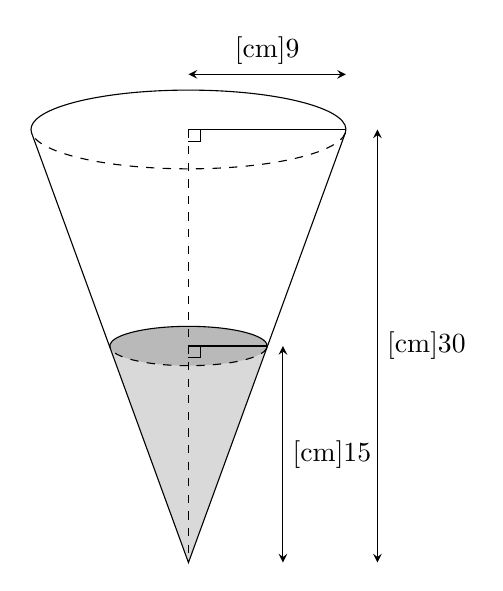
\begin{tikzpicture}[baseline={(T.base)},y=-1cm,>=stealth]
	\fill[gray!30] (1,2.75)--(0,5.5)--(-1,2.75);
	\fill[gray!55] (0,2.75) circle (1 and 0.25);
	\draw (5.22:2 and 0.5) arc (5.22:-185.22:2 and 0.5) ;
	\draw[dashed] (5.22:2 and 0.5) arc (5.22:174.88:2 and 0.5) ;
	\draw (5.22:2 and 0.5)--(0,5.5) --(174.88:2 and 0.5);
	\draw (2,0) --(0,0) (0.15,0)--(0.15,0.15)--(0,0.15);
	\draw[shift={(0,2.75)}] (1,0) --(0,0) (0.15,0)--(0.15,0.15)--(0,0.15);
	\draw[shift={(0,2.75)}] (5.22:1 and 0.25) arc (5.22:-185.22:1 and 0.25) ;
	\draw[shift={(0,2.75)},dashed] (5.22:1 and 0.25) arc (5.22:174.88:1 and 0.25) ;
	\draw[dashed](0,0)--(0,5.5);
	\draw[<->] (0,-0.7)--(2,-0.7)node[above,pos=0.5] (T){\np[cm]{9}};
	\draw[<->] (1.2,2.75)--(1.2,5.5)node[right,pos=0.5]{\np[cm]{15}};
	\draw[<->] (2.4,0)--(2.4,5.5)node[right,pos=0.5]{\np[cm]{30}};
\end{tikzpicture}

\item Léo décide d'utiliser son chapeau pour transporter les bonbons qu'il a récoltés pendant la fête d'Halloween. En arrivant chez lui, il constate que les bonbons atteignent le milieu de la hauteur de son chapeau. Il estime que sa récolte de bonbons n'a pas été bonne car il pense que le volume occupé par les bonbons représente moins de 15\,\% du volume total de son chapeau. Son estimation est-elle correcte ?
\end{enumerate}
